\section{Evaluation of Compositionally Embedded \ExT} \label{sec:evaluation}

In this section, we describe three applications of CP, compare them with
alternatives in other document languages, and evaluate the use of
compositionally embedded \ExT for the three applications.

\subsection{Minipedia} \label{sec:minipedia}

Minipedia is a mini document repository of states and cities, which reconstructs
a small portion of Wikipedia. Minipedia currently contains pages of the world's
ten smallest countries and their capitals, as well as a structured data file
storing all facts about them used for infoboxes. There are also pages consisting
of sorted tables of microstates by area or population, which are computed using
the information stored in the data file. Minipedia comprises over 4,000 lines of
code in total, most of which is accounted for by document pages. Among the rest,
the data file and \ExT libraries account for around 300 and 200 lines of code,
respectively.

\paragraph{Drawbacks of Wikipedia.}
Compared to our approach, Wikipedia and its markup language Wikitext have
several drawbacks, as partly mentioned in \autoref{sec:goals}:
\begin{itemize}
\item All data in Wikitext is in string format. Wikitext does not differentiate
      data types like \lstinline{Int}, \lstinline{Bool}, etc. This makes type
      errors remain uncaught in Wikipedia infoboxes. For example, in the infobox
      of a country, the population field can be changed to a non-numeric
      meaningless value, and Wikipedia will not warn the editor at all.
\item Statistical data is manually written on every Wikipedia page. This can
      easily result in data inconsistency for the same field across different
      pages, and even for different places on the same page. For example, the
      population size on a country page is often different from that in a
      statistical page listing all countries by population, owing to different
      data sources.
\item Wikitext provides user-defined templates as a reusable unit of document
      fragments. They can be parametrized and play a similar role to functions.
      However, they do not natively support general-purpose computation like
      recursion. Along with the Lua extension and parser functions, Wikitext
      offers some computational power to Wikipedia documents, but it is not as
      easy to use as \ExT is.
\end{itemize}

\paragraph{Type safety and data consistency.}
Minipedia has a structured data file containing the information of states and
cities, each piece of which is modeled as a record. The record types have been
shown in \autoref{sec:typing}. Every record for states or cities is type checked
against their corresponding types and collected in two arrays in the data file:

\noindent
\begin{minipage}{0.5\textwidth}
\begin{lstlisting}
tuvalu = {
  name       = "Tuvalu";
  area       = 26;
  population = 10645;
  -- and more fields
} : StateInfo;
states = [tuvalu; {- and more -}];
\end{lstlisting}
\end{minipage}%
\begin{minipage}{0.5\textwidth}
\begin{lstlisting}
funafuti = {
  name       = "Funafuti";
  area       = 2;
  population = 6320;
  -- and more fields
} : CityInfo;
cities = [funafuti; {- and more -}];
\end{lstlisting}
\end{minipage}
\smallskip

\noindent Such a centralized data file forces different documents to read from
the same data source and prevents data inconsistency. Not only infoboxes but
also computed documents like sorted lists of countries can be created using the
information from the data file. Moreover, if the area of Tuvalu, for example, is
assigned a string value, there will be a type error before rendering.

\paragraph{Writing Minipedia pages in \ExT.}
Writing Minipedia documents is enabled by the \ExT libraries shown in
\autoref{fig:diagram}. Different features of \ExT are defined in different
libraries, and we can import whatever libraries we want when writing a document.
For Minipedia, we only need HTML-related libraries. There are two modes for
document authoring in Minipedia: ``doc-only'' and ``program''. In the
``doc-only'' mode, with required libraries specified, documents are written
directly in \ExT without any wrapping code in CP, as shown in
\autoref{fig:example}. In the ``program'' mode, a document is created
programmatically in a mixture of CP and \ExT code. This mode makes
general-purpose computation easier to write in a document.

For example, a sorted table of the smallest countries by area demonstrates
general-purpose computation in the ``program'' mode. The program begins with an
\lstinline{open} directive, which imports definitions from the specified
libraries. We sort the array of countries imported from \lstinline{Database}
using a predefined function \lstinline{sort} and then iterate it to generate
\ExT code. As explained in \autoref{sec:sharing}, we use self-type annotations
to inject dependencies on the library commands. The intersection type
\lstinline{DocSig<T>&TableSig<T>} allows \ExT commands from both compositional
interfaces to be used in the trait \lstinline{doc}:

\begin{lstlisting}
open LibDoc;
open LibTable;
open Database;

sortedStates = sort states;

doc T = trait [self: DocSig<T>&TableSig<T>] => open self in {
  table = letrec rows (i: Int): T =
      if i == 0 then `\Trow[
        \Theader[No.]   \Theader[Country]      \Theader[Area (km^2)]
      ]` else let state = sortedStates!!(i-1) in `\rows(i-1) \Trow[
        \Tdata[\(i+1)]  \Tdata[\(state.name)]  \Tdata[\(state.area)]
      ]` in
  `\Tbody[ \rows(#sortedStates) ]`;
};
document = new doc @HTML , html , table;
document.table.html
\end{lstlisting}

\noindent
A table of the smallest countries by area rendered by the code above is shown in
\autoref{fig:minipedia-1}.

\begin{figure}
\begin{subfigure}{.5\textwidth}
\centering
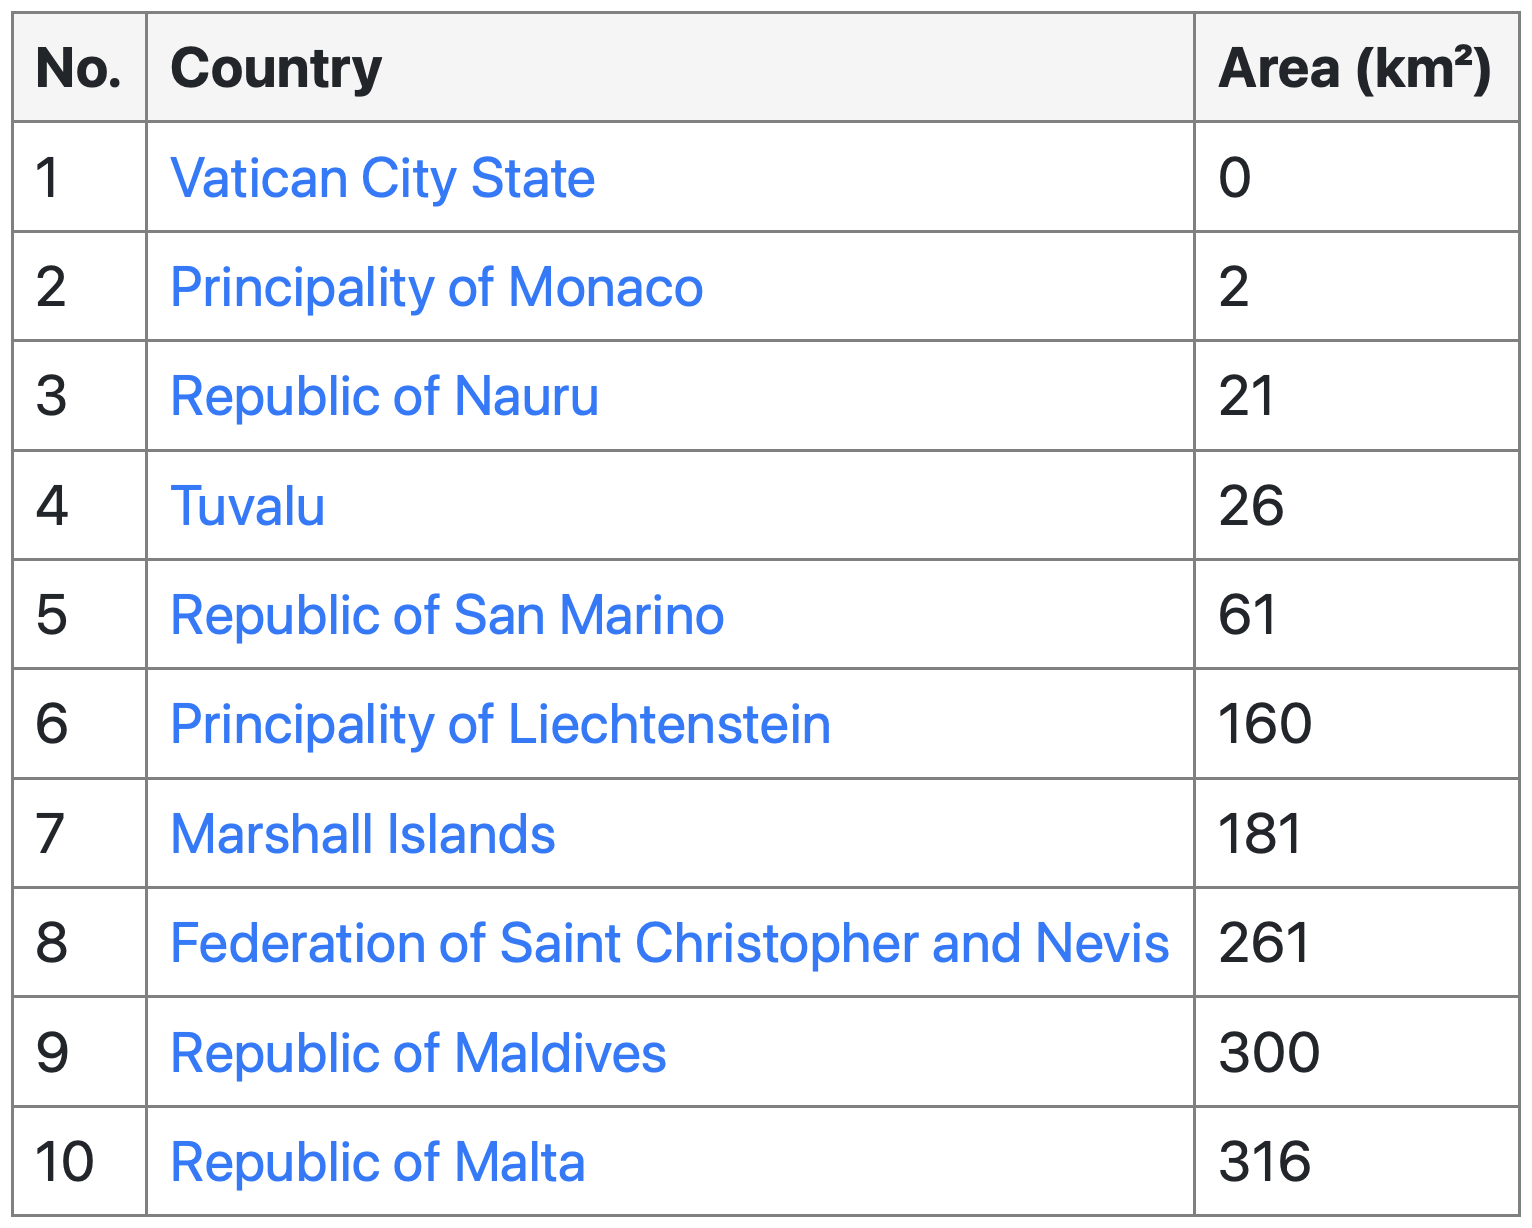
\includegraphics[width=\textwidth]{minipedia-1.png}
\caption{The smallest countries by area.}
\label{fig:minipedia-1}
\end{subfigure}%
\begin{subfigure}{.5\textwidth}
\centering
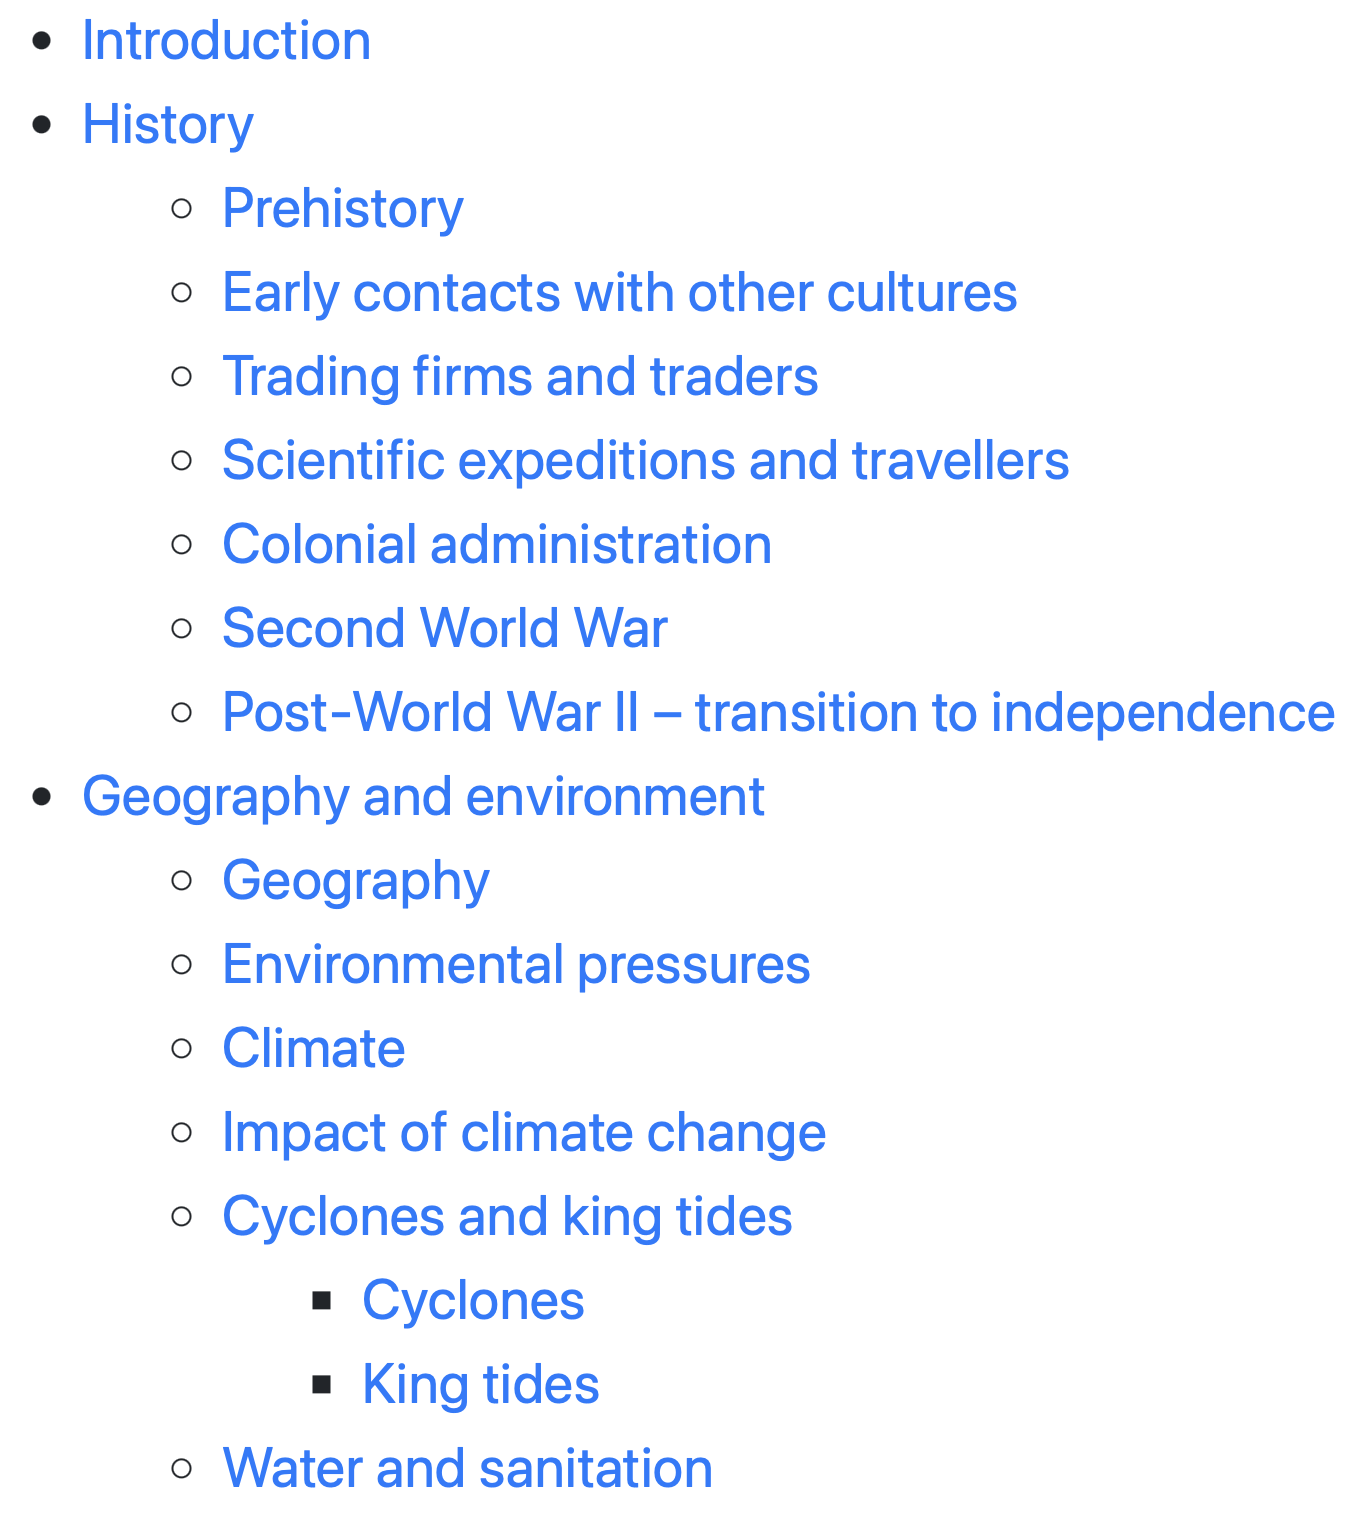
\includegraphics[width=.9\textwidth]{minipedia-2.png}
\caption{Table of contents of the Tuvalu page.}
\label{fig:minipedia-2}
\end{subfigure}
\caption{Screenshots of Minipedia pages.}
\end{figure}

\paragraph{Adding a table of contents (TOC).}
We have introduced how to write Minipedia pages using \ExT libraries, but now
let us go back and see how we implement a \ExT library. The library of TOC adds
a new command \lstinline{\Body[...]}, which prepends a TOC to the document body.
The difficulty here is that HTML rendering depends on the TOC, whereas the TOC
in turn depends on the HTML rendering of section (and sub$^n$section) titles. As
we have demonstrated in \autoref{sec:deps}, we can modularly tackle such complex
dependencies by refining the interface types:

\begin{lstlisting}
type ContentsSig<Element> = { Body: Element -> Element };
type TOC = { toc: String };

contents = trait implements ContentsSig<TOC => HTML> => {
  [self]@(Body e).html = self.toc ++ e.html;
};
toc = trait implements TextualSig<HTML => TOC> & ContentsSig<TOC> => {
  (Comp        l r).toc = l.toc ++ r.toc;
  (Section       e).toc = listItem 0 e.html;
  (SubSection    e).toc = listItem 1 e.html;
  (SubSubSection e).toc = listItem 2 e.html;
  (Body          e).toc = "<ul>" ++ e.toc ++ "</ul>";
                  _.toc = "";
};
\end{lstlisting}

\noindent With \lstinline{TOC} specified in \lstinline{ContentsSig<TOC => HTML>}
and the self-reference specified in \lstinline{[self]}, we can call
\lstinline{self.toc} to generate a TOC when rendering HTML. Similarly, we can
call \lstinline{e.html} when generating the TOC since the interface type is
refined. A minor remark is that \lstinline{listItem} is an auxiliary function to
generate an appropriate \lstinline{<li>} wrapping for a given nesting level.

An example of a TOC is shown in \autoref{fig:minipedia-2}. The TOC is generated
automatically from the section titles in the Tuvalu page. The TOC is a
compositional part of the document and is not hard-coded in the document body.
This is a good example of how to modularly handle dependencies in compositional
embeddings.

\subsection{Fractals and Sharing} \label{sec:fractal}

In the second application, we briefly introduce how to implement computational
graphics like fractals in \ExT with the help of linguistic reuse. Fractal
drawing is all about repeating the same pattern. This drives us to exploit
meta-language sharing to avoid redundant computation. We have implemented
several well-known fractals, such as the Koch snowflake, the T-square, and the
Sierpiński carpet. For the sake of simplicity, we take the Sierpiński carpet as
an example:

\begin{lstlisting}
fractal T C =
  trait [self: DocSig<T> & GraphicSig<T><C> & ColorSig<C> & Draw T C]
  implements Draw T C => open self in {
    draw {..} =
      let center = Rect { x = x + width/3; y = y + height/3;
                          width = width/3; height = height/3; color = White} in
      if level == 0 then center else
        let w = width/3 in let h = height/3 in let l = level-1 in
        let shared = draw { x = x; y = y; width = w; height = h; level = l } in
        `\Group(id)[
          \shared
            \Translate{ x = w; y = 0 }(shared)
              \Translate{ x = 2*w; y = 0 }(shared)
          \Translate{ x = 0; y = h }(shared)
            \center
              \Translate{ x = 2*w; y = h }(shared)
          \Translate{ x = 0; y = 2*h }(shared)
            \Translate{ x = w; y = 2*h }(shared)
              \Translate{ x = 2*w; y = 2*h }(shared)
        ]`
};
\end{lstlisting}

\noindent We make variables shared via the \lstinline{let} expressions in CP.
There are many uses in the code above but, among them, \lstinline{shared}
accelerates fractal generation the most. The variable \lstinline{shared} is
later used eight times to constitute the repeating patterns in the Sierpiński
carpet. \lstinline{\Translate} is a command declared in \lstinline{GraphicSig}
for geometric translations. With automatic linguistic reuse in \ExT, we only
need to generate a pattern once instead of repeating it eight times. Besides the
efficiency in generating fractals, our implementation of \lstinline{\Translate}
makes use of the \lstinline{<use>} element in SVG to avoid the exponential
growth of output. Therefore, the duplication of SVG elements is also eliminated.
These optimizations are available for free thanks to the linguistic reuse in
compositional embeddings.

A screenshot of the Sierpiński carpet with \lstinline{level = 4} is shown in
\autoref{fig:carpet}.

\begin{figure}
\begin{subfigure}{.4\textwidth}
\centering
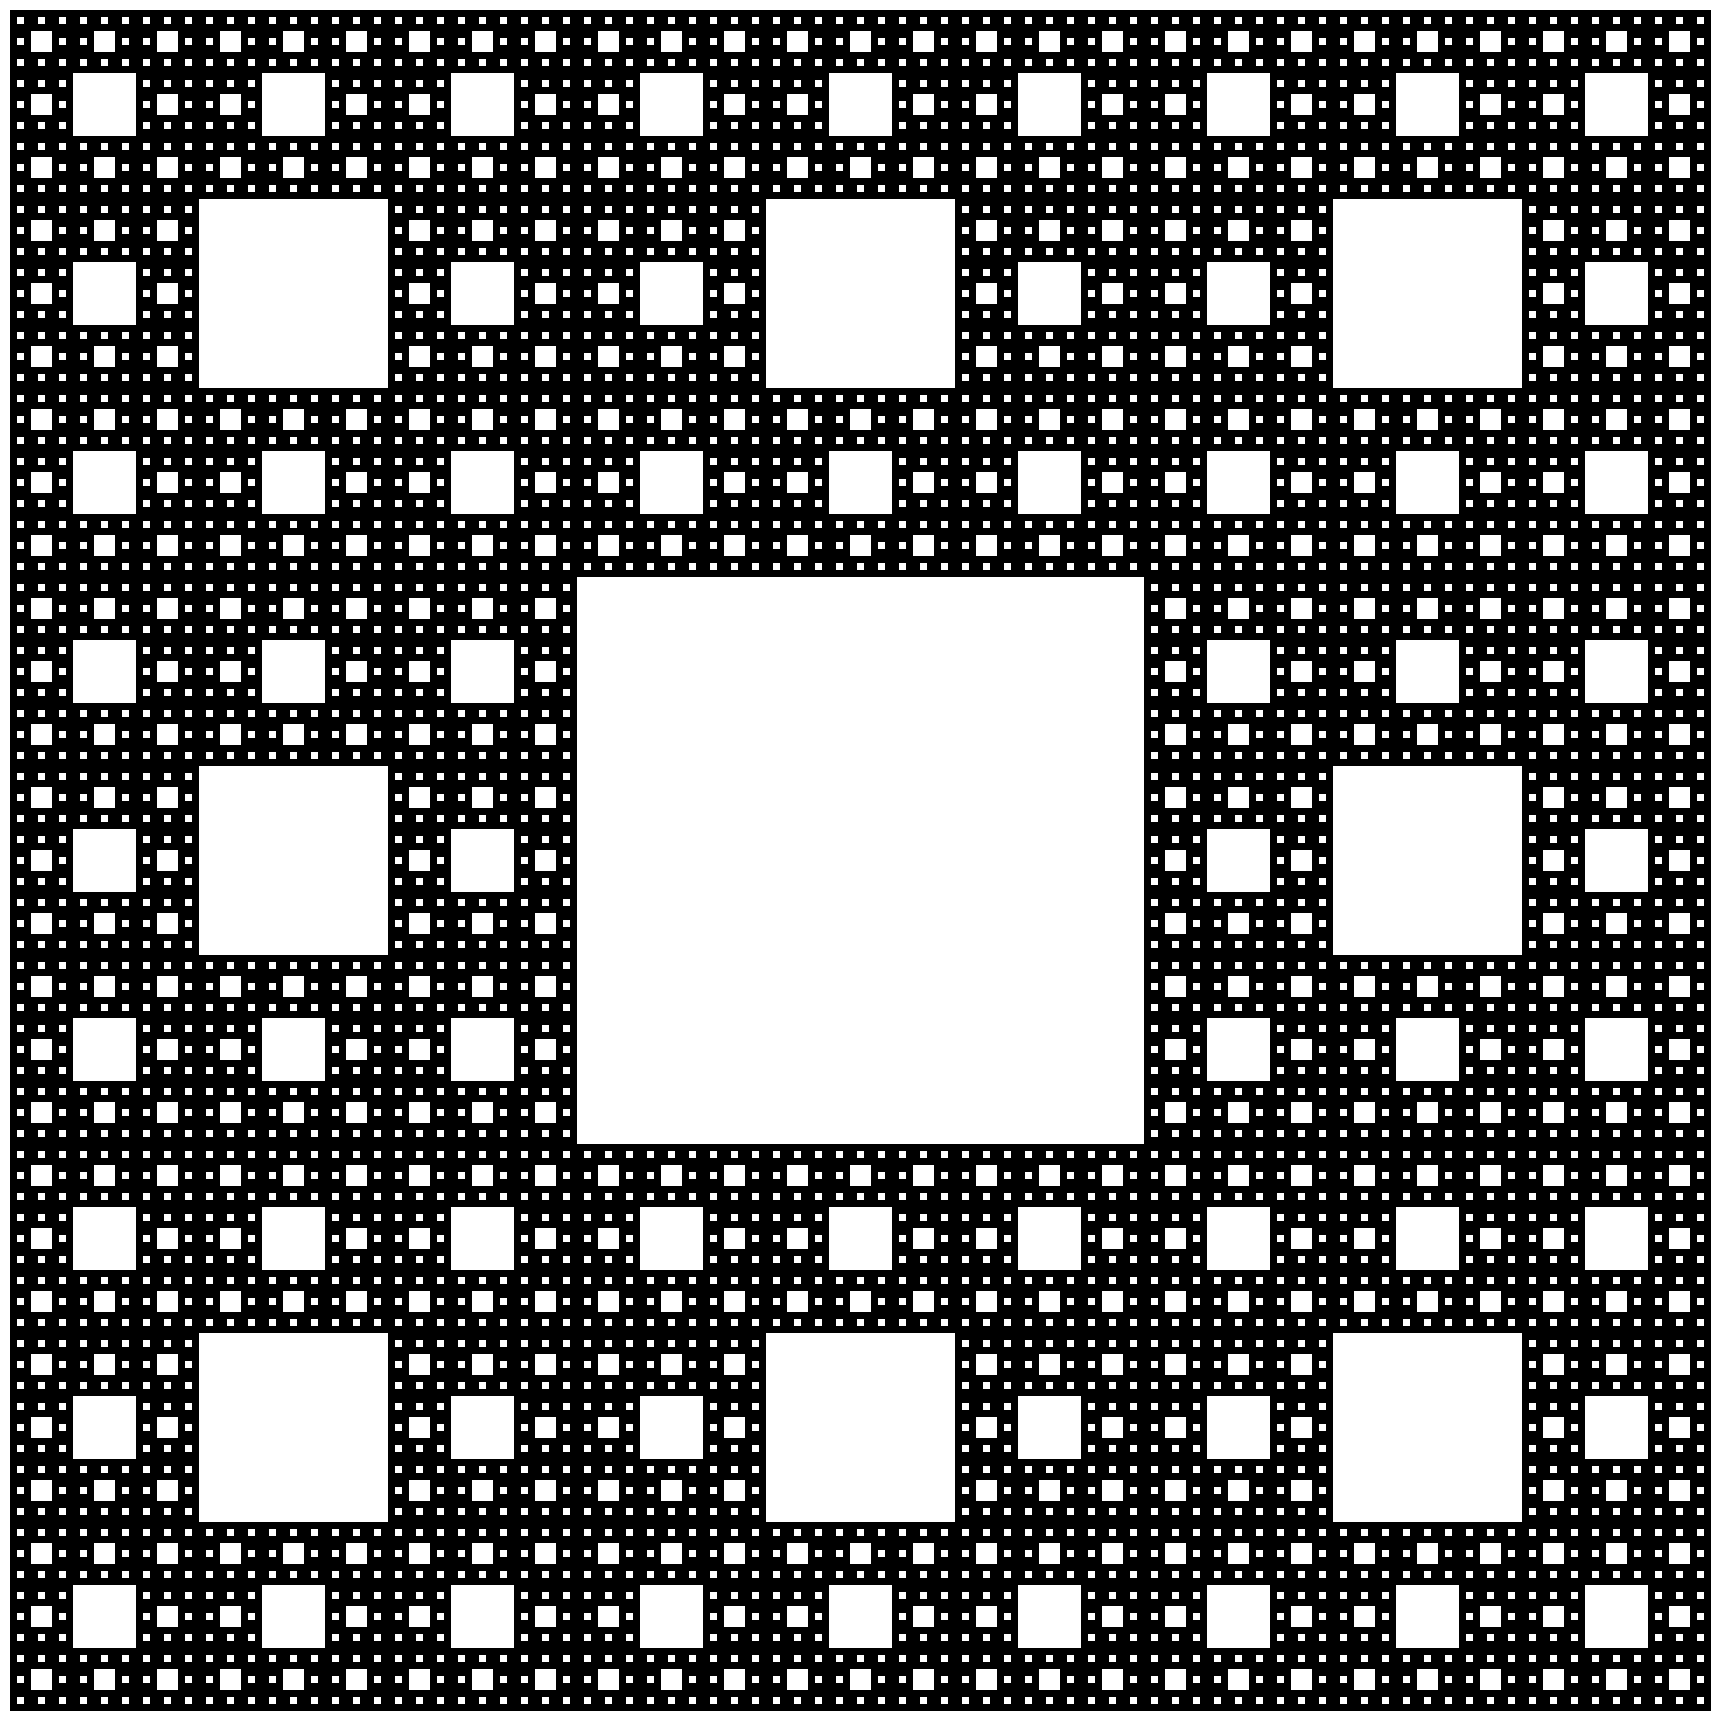
\includegraphics[width=.9\textwidth]{fractal.png}
\caption{Sierpiński carpet.}
\label{fig:carpet}
\end{subfigure}%
\begin{subfigure}{.6\textwidth}
\centering
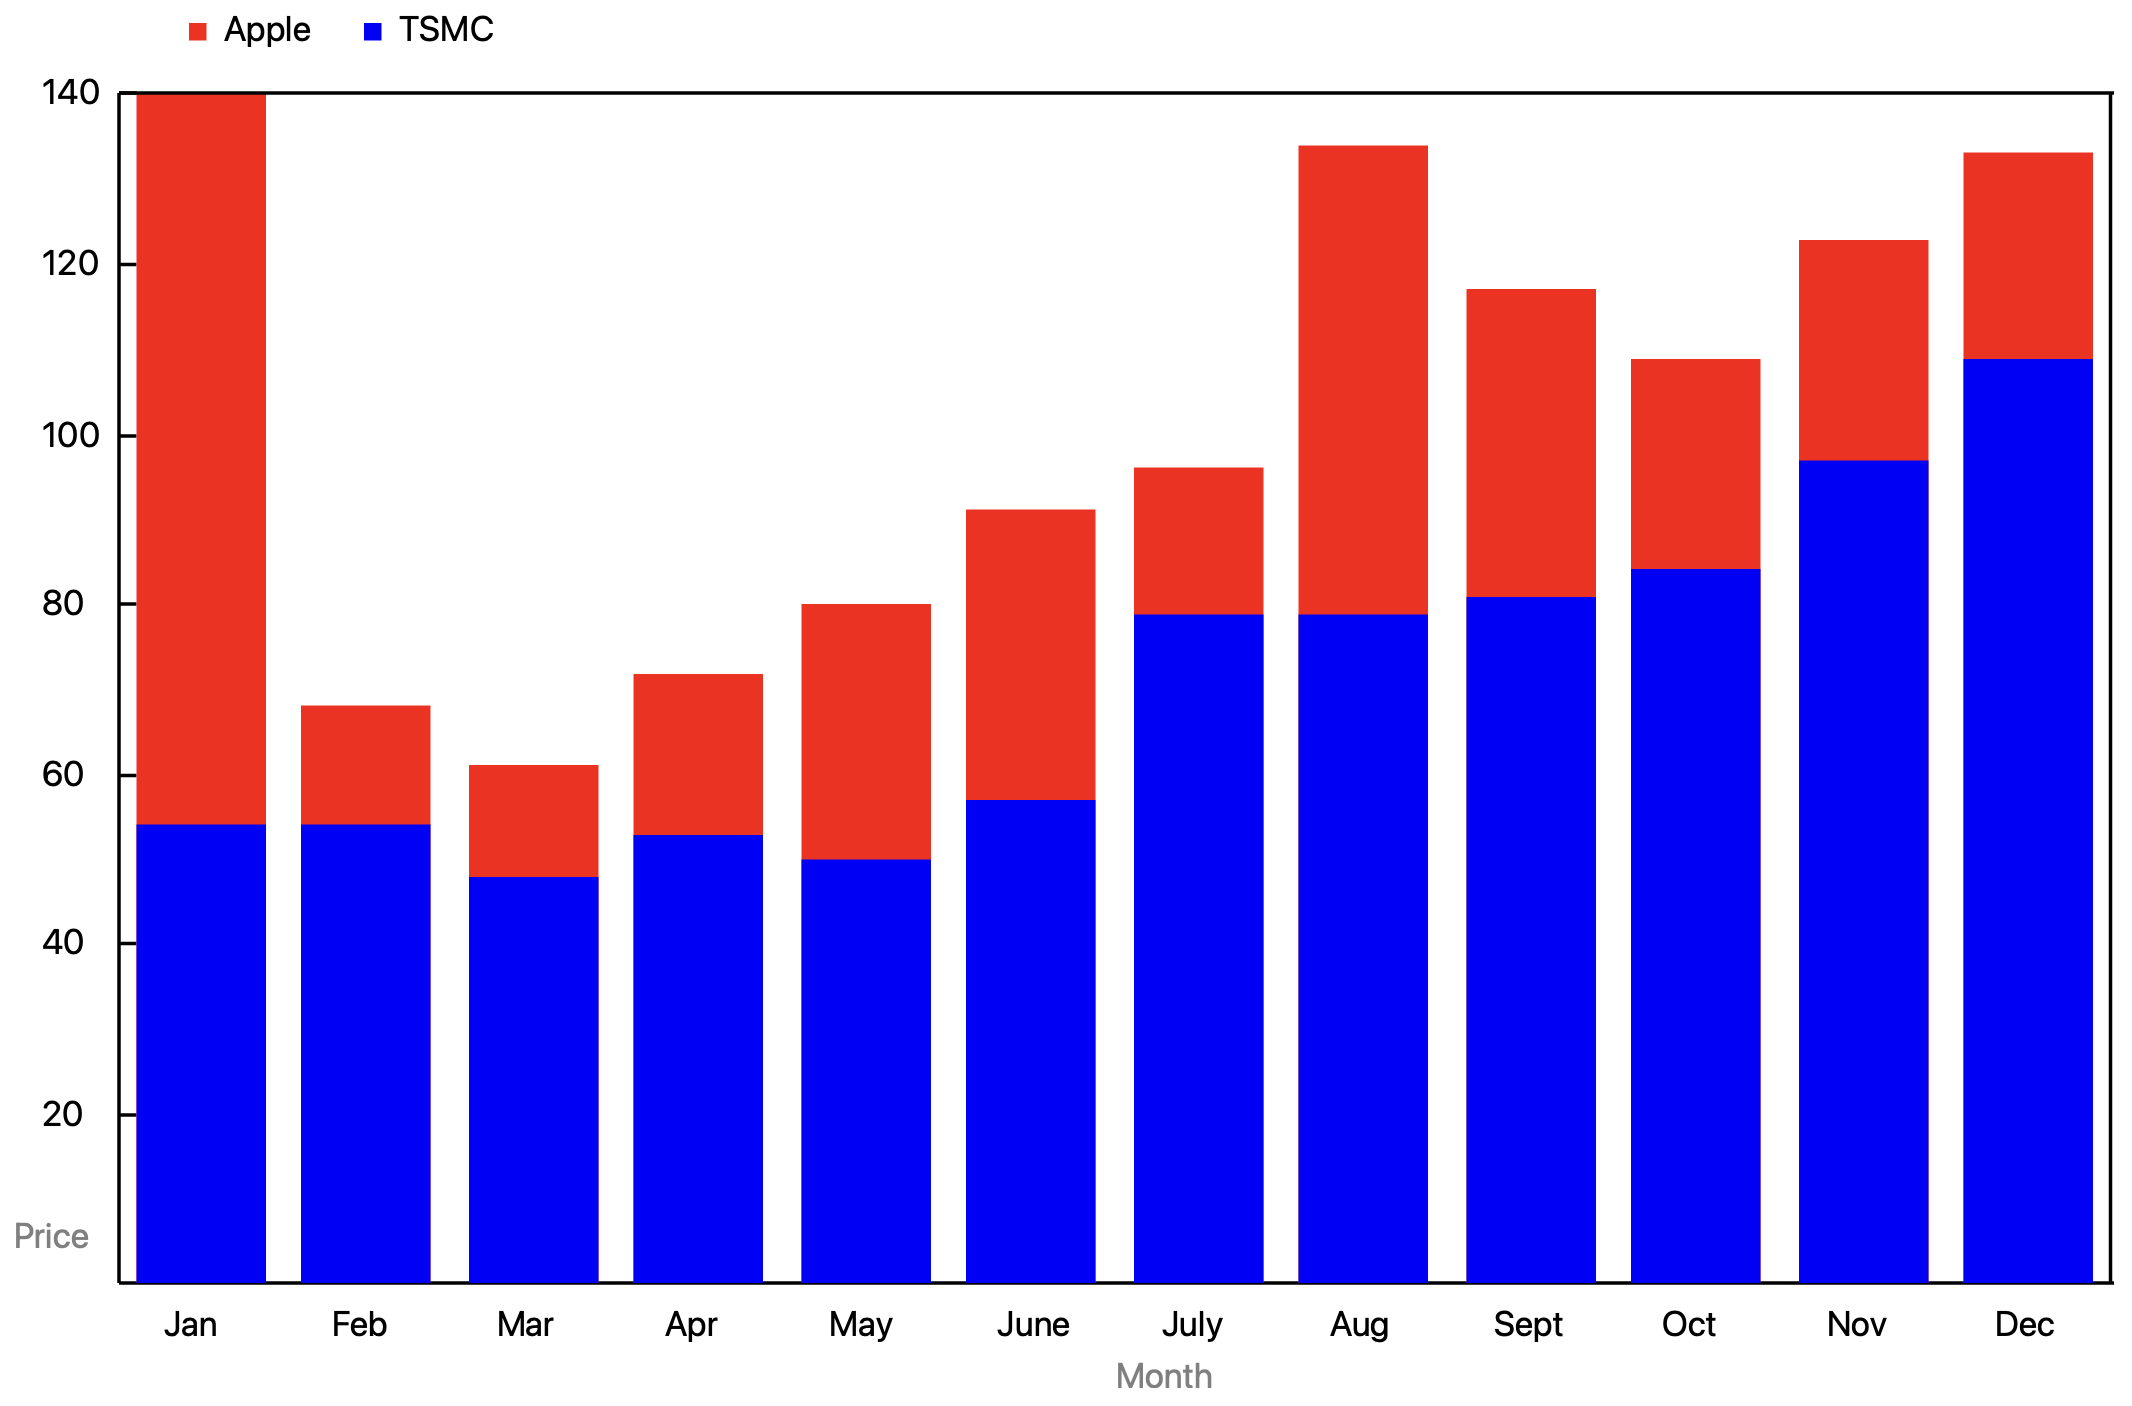
\includegraphics[width=.9\textwidth]{chart.png}
\caption{A bar chart of stock prices.}
\label{fig:chart}
\end{subfigure}
\caption{Screenshots of fractals and charts.}
\end{figure}

\subsection{Customizing Charts} \label{sec:charts}

In the last application, we illustrate how line charts and bar charts are
modularly rendered using external data. Charts can be rendered into a document
using the \ExT language and its support for vector graphics. What is interesting
about charts is that there are many alternative ways to present charts and
customize them. The flexibility of the CP language, in terms of modularity and
compositionality, is then very useful here. We will show how to adapt
traditional object-oriented design patterns for compositional embeddings when
modeling graphic components.

\paragraph{Charting stocks.}
Taking stock prices as an example, we have a separate file containing data from
big companies, as well as a few configuration items for chart rendering. The
configuration includes the choice between lines and bars, whether to show
borders or legends, what labels to display, and so on. Serving as an
infrastructure, a base chart is created with the drawing functions for the
caption and axes:

\begin{lstlisting}
type Base = { caption: HTML; xAxis: HTML; yAxis: HTML };
baseChart (data: [Data]) = trait implements Base => {
  caption = `...`;  xAxis = `...`;  yAxis = `...`;
};
\end{lstlisting}

\noindent
The simplified code above shows a rough sketch, where a base trait takes data as
its parameter and implements the base interface. However, it does not implement
the primary rendering function. As we have two options to visualize stock
prices, we leave the choice to the \textsc{Strategy}
pattern~\citep{gamma1995design}.

\paragraph{\textsc{Strategy} pattern.}
Since the configuration is unknown until run time, the rendering strategy cannot
be hard-coded in the base trait. Instead, we define two strategy traits
implementing the rendering, respectively for lines and bars. They constitute two
variants of the base chart. It is not the programmer but the configurator that
decides which variant of charts should be rendered. In the original
\textsc{Strategy} pattern, a chart object delegates to a desired strategy
object, to which its mutable field points. That mutable field can be changed
from clients who use the chart. In CP, we just need to merge the base trait with
the strategy we want, without the need for mutable references:

\begin{lstlisting}
type Render = { render: HTML };
lineStrategy = trait [self: Base] implements Render => open self in {
  render = let lines = ... in `\xAxis \yAxis \lines \caption`
};
barStrategy = trait [self: Base] implements Render => open self in {
  render = let bars = ... in `\xAxis \yAxis \bars \caption`
};
chart = baseChart data , if config.line then lineStrategy else barStrategy;
\end{lstlisting}

\noindent
After merging, \lstinline{chart} is still a \emph{reusable trait}. This is
impossible in traditional object-oriented languages, like Java, because they
lack a dynamic way to compose classes at run time. In contrast, such a dynamic
trait composition is ubiquitous in CP. It is also easy to add a new strategy,
like switching to pie charts, and merge the base trait with the new one instead.
If a client forgets to pick any strategy, the type checker will notify them
because the trait types before and after merging are different. Moreover,
another advantage of our approach over the original strategy pattern is that the
self-type annotations make methods in the base trait accessible to strategy
traits. So \lstinline{caption}, \lstinline{xAxis} and \lstinline{yAxis} are
directly shared with strategies, requiring no extra effort to pass them as
arguments when delegating. This remedies the ``communication overhead between
Strategy and Context'' caused by the original \textsc{Strategy}
pattern~\citep{gamma1995design}.

\paragraph{\textsc{Decorator} pattern.}
Besides the \textsc{Strategy} pattern, the \textsc{Decorator}
pattern~\citep{gamma1995design} is also adapted for CP. Since decorations are
also determined by external configuration at run time, we need a modular way to
add additional drawing processes to the chart trait dynamically. When multiple
decorators are enabled, their functionalities should be added. In the original
\textsc{Decorator} pattern, the decorator class should inherit the chart class
and be instantiated with a reference to a chart object. The decorator will store
the chart object as a field and forward all methods to it. In concrete
decorators, the rendering function will be overridden to add decorations. The
decorator pattern sounds complicated in traditional object-oriented programming,
but the same goal can be achieved easily in CP using the \emph{dynamic
inheritance} provided by CP:

\begin{lstlisting}
type Chart = Base & Render;
borderDecorator (chart: Trait<Chart>) = trait [self: Chart]
                                        implements Chart inherits chart => {
  override render = let sr = super.render in let border = ... in `\sr \border`
};
legendDecorator (chart: Trait<Chart>) = trait [self: Chart]
                                        implements Chart inherits chart => {
  override caption = let legends = ... in `\legends`
};
chart' = if config.border then borderDecorator chart else chart;
chart'' = if config.legend then legendDecorator chart' else chart';
\end{lstlisting}

\noindent
A decorator takes a chart trait as the argument and creates another trait
inheriting it dynamically. In the implementation, we can override any methods as
usual, and static type safety is still guaranteed. It is worth noting that, in
\lstinline{legendDecorator}, only \lstinline{caption} is overridden while
\lstinline{render} is just inherited. In the original \textsc{Decorator}
pattern, \lstinline{render} will never be conscious of the overridden
\lstinline{caption} since the decorator hands over control to \lstinline{chart}
after forwarding \lstinline{render}. This is partly why \citet{gamma1995design}
warn readers that ``a decorator and its component aren't identical''. However,
in CP, \lstinline{chart.render} can access the overridden \lstinline{caption}
through the late-bound self-reference. This solution makes our code clean and
easy to maintain.

A bar chart of stock prices with borders and legends is shown in
\autoref{fig:chart}.

\paragraph{True delegation via trait composition.}
The chart application shows how other aspects of the modularity of CP are
helpful to create highly customizable DSLs. We have shown how CP adapts and
simplifies object-oriented design patterns. In general, we avoid complicated
class hierarchies in the original versions and replace them with relatively
simple trait composition. It showcases that we can get rid of verbose design
patterns if a proper language feature fills in the gap. In both patterns,
component adaptation is needed at run time, so delegation is at the heart of the
challenges.
